\section{Auswertung}
\label{sec:auswertung}

Alle in der Auswertung angegebenen Größen sind stets auf die erste signifikante
Stelle des Fehlers gerundet. Setzt sich eine Größe über mehrere Schritte aus
anderen Größen zusammen, so wird erst am Ende gerundet, um Fehler zu vermeiden.
Zur Auswertung wird die Programmiersprache \texttt{python (Version 3.5.2)} mit
den Bibliothekserweiterungen \texttt{numpy}~\cite{numpy},
\texttt{scipy}~\cite{scipy} und \texttt{matplotlib}~\cite{matplotlib} verwendet.

\subsection{Kompensation des Erdmagnetfeldes}
Die Vertikalfeldspule wird verwendet um die vertikale Komponente des
Erdmagnetfeldes zu kompensieren. Das Magnetfeld eines Helmholtzspulenpaares
beträgt in Abhängigkeit des Spulenstroms~$I$, der Windungszahl pro Spule~$N$ und
dem Spulenradius~$R$
%
\begin{equation}
  B = \mu_0\frac{8\cdot IN}{\sqrt{125}\cdot R}
  \label{eq:bfeld}
\end{equation}
%
Für die gegebene Vertikalspule gilt~$N=20$ und $R=\SI{11.735}{\centi\metre}$.
Bei einem eingestellten Spulenstrom von~$\SI{245}{\milli\ampere}$ wird der
Einfluss des Erdmagnetfeldes minimal. Daraus ergibt sich die vertikale
Komponente des Erdmagnetfeldes zu~$B_{\bot}=\SI{37.55}{\micro\tesla}$.

\subsection{Bestimmung der Landé-Faktoren und der Kernspins}
Tabelle~\ref{tab:magnetfeld} zeigt die RF-Frequenzen zusammen mit den
eingestellten Strömen für die Horizontalfeld- und die Sweepspule, bei denen die
Transparenz der Zelle ein lokales Minimum hat. Aus den Strömen wird das
Gesamtmagnetfeld~$B$ berechnet, wobei Gleichung~\eqref{eq:bfeld} verwendet wird.
Für die Horizontalfeldspule gilt~$N=154$ und~$R=\SI{15.79}{\centi\metre}$. Die
Kenngrößen der Sweepspule sind durch~$N=11$ und~$R=\SI{16.39}{\centi\metre}$
gegeben.
%
\begin{table}[htb]
  \centering
  \caption{Gemessene Stromstärken und berechnetes Magnetfeld für~$\ce{^87Rb}$
  und~$\ce{^85Rb}$ bei eingestellter Hochfrequenz.}
  \begin{tabular}{S[table-format=4.0]|
                  S[table-format=3.0]
                  S[table-format=3.0]
                  S[table-format=3.2]|
                  S[table-format=3.0]
                  S[table-format=3.0]
                  S[table-format=3.2]}
    \toprule
    & \multicolumn{3}{c}{\ce{^87Rb}} & \multicolumn{3}{c}{\ce{^85Rb}} \\
    {$\displaystyle\frac{\nu}{\si{\kilo\hertz}}$} &
    {$\displaystyle\frac{I_{\symup{H}}}{\si{\milli\ampere}}$} &
    {$\displaystyle\frac{I_{\symup{S}}}{\si{\milli\ampere}}$} &
    {$\displaystyle\frac{B}{\si{\micro\tesla}}$} &
    {$\displaystyle\frac{I_{\symup{H}}}{\si{\milli\ampere}}$} &
    {$\displaystyle\frac{I_{\symup{S}}}{\si{\milli\ampere}}$} &
    {$\displaystyle\frac{B}{\si{\micro\tesla}}$} \\
    \midrule
     100 &   0 & 475 &  28.67 &   0 & 595 &  35.91 \\
     200 &  30 & 320 &  45.62 &  30 & 560 &  60.10 \\
     300 &  30 & 550 &  59.50 &  30 & 900 &  80.62 \\
     400 &  66 & 265 &  73.87 &  66 & 740 & 102.54 \\
     500 &  81 & 264 &  86.97 &  81 & 855 & 122.63 \\
     600 & 102 & 205 & 101.82 & 102 & 905 & 144.07 \\
     700 & 126 &  87 & 115.75 & 126 & 912 & 165.53 \\
     800 & 126 & 324 & 130.05 & 165 & 716 & 187.91 \\
     900 & 159 & 122 & 146.80 & 195 & 633 & 209.21 \\
    1000 & 165 & 244 & 159.42 & 210 & 761 & 230.09 \\
    \bottomrule
  \end{tabular}
  \label{tab:magnetfeld}
\end{table}
%
Eine lineare Regression des Magnetfeldes gegen die eingestellte Frequenz liefert
%
\begin{align}
  B_{87}&=\SI{1.441(11)e-7}{\tesla\per\kilo\hertz}\cdot\nu
  +\SI{1.56(7)e-5}{\tesla} \\
  B_{85}&=\SI{2.144(9)e-7}{\tesla\per\kilo\hertz}\cdot\nu
  +\SI{1.59(6)e-5}{\tesla}
\end{align}
%
\begin{figure}[htb]
  \centering
  \includegraphics[width=0.75\textwidth]{analysis/magnetfeld.pdf}
  \caption{Horizontales Magnetfeld aufgetragen gegen die Frequenz.}
  \label{fig:magnetfeld}
\end{figure}
%
Gemäß Gleichung~\eqref{eq:übergangsenergie} folgen daraus die Landé-Faktoren
%
\begin{align}
  g_{\text{F,87}}&=\num{0.496(4)} \\
  g_{\text{F,85}}&=\num{0.3332(15)}
\end{align}
%
Die Bestimmung der Landé-Faktoren~$g_{\symup{F}}$ ermöglicht die Berechnung der
Kernspins der beiden Rubidiumisotope. Dazu wird zunächst mit Hilfe von
Gleichung~\eqref{eq:gj} der Landé-Faktor~$g_{\symup{J}}$ berechnet.
Mit~$S=\sfrac{1}{2}$,~$L=0$ und~$J=\sfrac{1}{2}$
folgt~$g_{\symup{J}}=\num{2.0023}$. Für den Kernspin gilt
%
\begin{equation*}
  I=\frac{g_{\symup{J}}}{2g_{\symup{F}}}-\frac{1}{2}
\end{equation*}
%
Daraus folgen
%
\begin{align}
  I_{87}&=\num{1.520(16)} \\
  I_{85}&=\num{2.505(13)}
\end{align}

\subsection{Bestimmung des Isotopenverhältnisses}
Abbildung~\ref{fig:signalbild} zeigt ein typisches Signalbild bei einer
Hochfrequenz von~$\SI{100}{\kilo\hertz}$. Dabei entspricht das
Amplitudenverhältnis der beiden beobachteten Transparenzminima dem
Isotopenverhältnis der untersuchten Probe.
%
\begin{equation}
  \frac{N\left(\ce{^85Rb}\right)}{N\left(\ce{^87Rb}\right)}
  =\frac{\num{4.4(2)}}{\num{2.2(2)}}
  =\num{2.0(2)}
\end{equation}
%
Die angegebenen Fehler resultieren aus einer Ungenauigkeit beim Ablesen der
Amplituden und entsprechen dem Abstand zwischen zwei Hilfsgitterlinien.
%
\begin{figure}[htb]
  \centering
  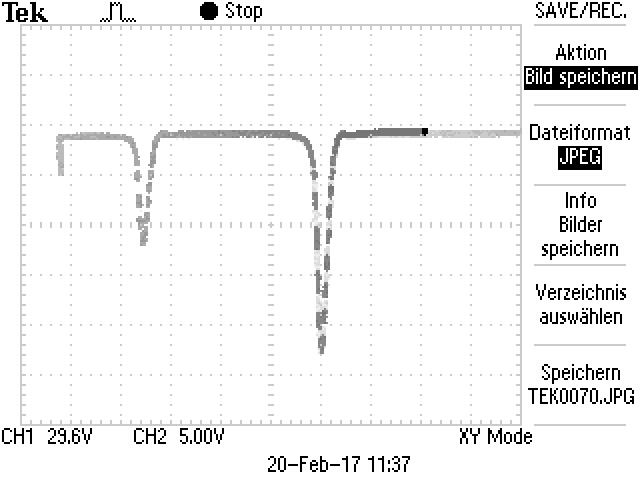
\includegraphics[width=0.75\textwidth]{analysis/signalbild.png}
  \caption{Oszilloskopbild eines typischen Signals
  bei~$\SI{100}{\kilo\hertz}$.}
  \label{fig:signalbild}
\end{figure}
%
\subsection{Untersuchung des quadratischen Zeeman-Effektes}
Im Folgenden wird der Einfluss des quadratischen Zeeman-Effekte untersucht. Dazu
wird die Formel
%
\begin{equation}
  U_{\symup{HF}}=g_{\symup{F}}\mu_{\symup{B}}B
  +g_{\symup{F}}^2\mu_{\symup{B}}^2B^2
  \frac{(1-2M_{\symup{F}})}{\symup{\Delta}E_{\symup{Hy}}}-\ldots
  \label{eq:zeemanenergie}
\end{equation}
%
betrachtet, wobei für eine obere Abschätzung das größte verwendete Magnetfeld
eingesetzt und~$M_{\symup{F}}=0$ gesetzt wird. Die Hyperfeinstrukturaufspaltung
des Grundzustandes ist durch
%
\begin{align}
  \symup{\Delta}E_{\text{Hy,87}}&=\SI{4.53e-24}{\joule} \\
  \symup{\Delta}E_{\text{Hy,85}}&=\SI{2.01e-24}{\joule}
\end{align}
%
gegeben. Für die Zeeman-Energie folgt dann in linearer Näherung
%
\begin{align}
  U_{\text{HF,87,linear}}&=\SI{7.33(6)e-28}{\joule} \\
  U_{\text{HF,85,linear}}&=\SI{7.110(31)e-28}{\joule}
\end{align}
%
und in quadratischer Näherung
%
\begin{align}
  U_{\text{HF,87,quadratisch}}&=\SI{1.186(18)e-31}{\joule} \\
  U_{\text{HF,85,quadratisch}}&=\SI{2.515(22)e-31}{\joule}
\end{align}
%
\subsection{Untersuchung der transienten Effekte}
%
\begin{figure}[htb]
  \centering
  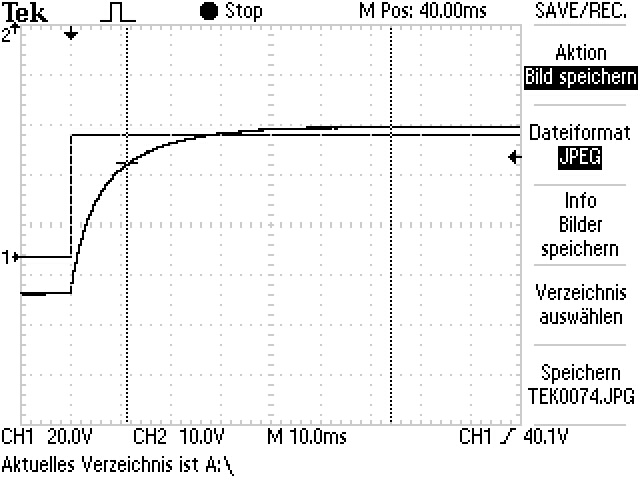
\includegraphics[width=0.75\textwidth]{analysis/anstieg.png}
  \caption{Oszilloskopbild bei angelegter Rechteckspannung.}
  \label{fig:anstieg}
\end{figure}
%
Abbildung~\ref{fig:anstieg} zeigt den exponentiellen Anstieg der Transparenz
der Zelle auf der~$\ce{^85Rb}$-Resonanz beim Anlegen einer Rechteckspannung.
Die aufgenommenen Messwerte zur Untersuchung der Abhängigkeit von
Schwingungsperiode und angelegter Hochfrequenzamplitude sind in
Tabelle~\ref{tab:periodendauer} aufgeführt. Die Anpassung von
Hyperbelfunktionen der Form
%
\begin{equation}
  T=a+\frac{b}{U-c}
\end{equation}
%
an die Messwerte liefert
%
\begin{align}
  T_{87}&=\SI{0.021(10)}{\milli\second}
  +\frac{\SI{2.18(6)}{\milli\second\volt}}{U-\SI{0.000(24)}{\volt}} \\
  T_{85}&=\SI{0.043(11)}{\milli\second}
  +\frac{\SI{3.10(6)}{\milli\second\volt}}{U-\SI{0.049(17)}{\volt}}
\end{align}
%
Es folgt das Verhältnis
%
\begin{equation}
  \frac{b_{85}}{b_{87}}=\frac{\num{3.10(6)}}{\num{2.18(6)}}=\num{1.42(5)}
\end{equation}
%
\begin{table}[htb]
  \centering
  \caption{Gemessene Periodendauern für~$\ce{^87Rb}$ und~$\ce{^85Rb}$ bei
  eingestellter Hochfrequenzamplitude.}
  \begin{tabular}{S[table-format=1.3]
    S[table-format=1.3]
    S[table-format=1.3]|
    S[table-format=1.3]
    S[table-format=1.3]
    S[table-format=1.3]}
    \toprule
    {$\displaystyle\frac{U}{\si{\volt}}$} &
    {$\displaystyle\frac{T_{87}}{\si{\milli\second}}$} &
    {$\displaystyle\frac{T_{85}}{\si{\milli\second}}$} &
    {$\displaystyle\frac{U}{\si{\volt}}$} &
    {$\displaystyle\frac{T_{87}}{\si{\milli\second}}$} &
    {$\displaystyle\frac{T_{85}}{\si{\milli\second}}$} \\
    \midrule
    1.000 & 2.20  & 3.30  & 6.000 & 0.376 & 0.553 \\
    2.000 & 1.12  & 1.64  & 7.000 & 0.324 & 0.480 \\
    3.000 & 0.756 & 1.09  & 8.000 & 0.285 & 0.422 \\
    4.000 & 0.570 & 0.825 & 9.000 & 0.271 & 0.398 \\
    5.000 & 0.448 & 0.660 & 9.756 & 0.263 & 0.385 \\
    \bottomrule
  \end{tabular}
  \label{tab:periodendauer}
\end{table}
%
\begin{figure}[htb]
  \centering
  \includegraphics[width=0.75\textwidth]{analysis/periodendauer.pdf}
  \caption{Periodendauer aufgetragen gegen die Hochfrequenzamplitude.}
  \label{fig:periodendauer}
\end{figure}
